\chapter{Resultados}
\label{cap:resultados}

\section{Alcance de los resultados}

Este capítulo informa identidades analíticas, contrastes confirmatorios sobre 13\,500 ejecuciones, una sensibilidad de ingeniería con 40\,500 trayectorias (sección~\ref{sec:engineering-sensitivity}) y una comparación reservada de mapas reducidos afines e híbridos sobre 9\,600 trayectorias (sección~\ref{sec:hybrid-results}). El protocolo confirmatorio se describe en el capítulo~\ref{cap:metodologia}. Los resultados de hipótesis y evaluación de modelos son sintéticos: provienen de un micromundo sin datos de mercado y sin comisiones. En la sección~\ref{sec:dex-pilot-results} se informa un piloto separado de disponibilidad de datos DEX; es solo descriptivo y no valida externamente el modelo ni las hipótesis. La ejecución confirmatoria tiene el identificador \code{\RunID}; sus sumas de verificación y el comando que la regenera figuran en el anexo~\ref{cap:anexos}.

\section{Resultados analíticos: profundidad e impacto}
\label{sec:res-analitico}

Para una venta fija de $q=500$ unidades de $X$, el impacto $I(q,\kappa x)$ de la ecuación~\eqref{eq:impacto} crece al reducir la reserva (tabla~\ref{tab:impacto}). Con $x=10\,000$, reducir la reserva a la cuarta parte multiplica el impacto por 3.7 y el deslizamiento por 3.5.

\begin{table}[htbp]
\centering
\caption{Impacto de una venta de $q=500$ unidades según la reserva (resultado analítico).}
\label{tab:impacto}
\small
\begin{tabular}{@{}rrrr@{}}
\toprule
Factor de reserva & Reserva $x$ & Impacto $I$ & Deslizamiento (\%) \\
\midrule
1.00 & 10\,000 & 0.09758 & 4.76 \\
0.75 & 7500 & 0.12908 & 6.25 \\
0.50 & 5000 & 0.19062 & 9.09 \\
0.25 & 2500 & 0.36464 & 16.67 \\
\bottomrule
\end{tabular}
\end{table}

La figura~\ref{fig:impacto} muestra la curva completa. Con $I(q,\kappa x)=2\log(1+q/(\kappa x))$ y $\kappa<1$ se cumple $I(q,\kappa x)>I(q,x)$ para todo $q>0$, y la derivada de la ecuación~\eqref{eq:dI} es negativa. Este resultado no se contrasta estadísticamente: es una consecuencia algebraica de la regla de producto constante y funciona como control de la implementación (verificación 8 del anexo).

\begin{figure}[htbp]
\centering
\begin{tikzpicture}
\begin{axis}[width=0.78\textwidth,height=6cm,xlabel={Factor de reserva $\kappa$},ylabel={Impacto logarítmico $I$},grid=major,xmin=0.1,xmax=1.05]
\addplot[thick,blue!70!black] table[col sep=comma,x=reserve_factor,y=log_impact] {\datadir/impact_curve.csv};
\end{axis}
\end{tikzpicture}
\caption{Impacto logarítmico de una venta de $q=500$ unidades según el factor de reserva.}
\label{fig:impacto}
\end{figure}

\section{Panorama de las condiciones}

La tabla~\ref{tab:resumen} resume las cinco condiciones, con 2700 ejecuciones cada una (300 semillas por 9 celdas). Las cuatro primeras condiciones son primarias; E1-máx es una extrapolación fuera de los niveles contrastados y no entra en la inferencia.

\begin{table}[htbp]
\centering
\caption{Resumen de las condiciones de confirmación (2700 ejecuciones por condición).}
\label{tab:resumen}
\small
\begin{tabular}{@{}lrrrrrr@{}}
\toprule
Condición & Área $A$ & Resp. máx. $M$ & Recup. & Retorno\,$^{a}$ & Prof. mín. & Retiro \\
\midrule
E0 & 2.363 & 0.1012 & 4.6\,\% & 20.47 & 11667 & 0\,\% \\
E1-baja & 1.056 & 0.1305 & 56.8\,\% & 14.82 & 11667 & 0\,\% \\
E1-alta & 0.100 & 0.1220 & 100.0\,\% & 2.54 & 11667 & 0\,\% \\
E3 & 0.180 & 0.1335 & 96.6\,\% & 4.27 & 6417 & 100\,\% \\
E1-máx & 0.005 & 0.1197 & 100.0\,\% & 1.22 & 11667 & 0\,\% \\
\bottomrule
\multicolumn{7}{@{}l}{\footnotesize $^{a}$ Media restringida con censura en 21 ticks.}
\end{tabular}
\end{table}

El error pico medio es $0.176$ en E0, $0.127$ en E1-baja, $0.064$ en E1-alta, $0.073$ en E3 y $0.008$ en E1-máx. Ninguna orden estuvo limitada por capital en las 13\,500 ejecuciones.

\begin{figure}[htbp]
\centering
\begin{tikzpicture}
\begin{axis}[width=0.9\textwidth,height=6.4cm,xlabel={Tick},ylabel={$|d_t|$ medio},grid=major,legend pos=north east,legend style={font=\scriptsize},xmin=0,xmax=20,ymin=0]
\addplot[thick,red!70!black] table[col sep=comma,x=tick,y=mean_abs_excess,restrict expr to domain={\thisrow{series_id}}{10:10}] {\datadir/trajectories.csv};
\addplot[thick,orange!85!black] table[col sep=comma,x=tick,y=mean_abs_excess,restrict expr to domain={\thisrow{series_id}}{20:20}] {\datadir/trajectories.csv};
\addplot[thick,blue!70!black] table[col sep=comma,x=tick,y=mean_abs_excess,restrict expr to domain={\thisrow{series_id}}{30:30}] {\datadir/trajectories.csv};
\addplot[thick,dashed,green!50!black] table[col sep=comma,x=tick,y=mean_abs_excess,restrict expr to domain={\thisrow{series_id}}{40:40}] {\datadir/trajectories.csv};
\legend{E0,E1-baja,E1-alta,E3}
\end{axis}
\end{tikzpicture}
\caption{Exceso de error medio $|d_t|$ por tick, promediado sobre todas las celdas y semillas.}
\label{fig:trayectorias}
\end{figure}

\section{H1: el arbitraje activo reduce el exceso de error}
\label{sec:res-h1}

El contraste primario compara E1-alta con E0. La diferencia media del área de exceso es $\Delta_1=-2.263$ (mediana $-2.078$; intervalo del 95\,\% $[-2.345,\,-2.182]$) y el $p$ unilateral con corrección de Holm es $1.5\times10^{-4}$; las 300 semillas van en la dirección prevista (tabla~\ref{tab:inferencia}). Se rechaza la hipótesis nula. La comparación de capacidades (E1-alta frente a E1-baja) arroja $\Delta=-0.956$ (intervalo $[-1.003,\,-0.909]$), también en las 300 semillas, de modo que la capacidad gradúa el efecto y no solo su presencia.

\begin{table}[htbp]
\centering
\caption{Inferencia confirmatoria (300 semillas, contrastes pareados por semilla).}
\label{tab:inferencia}
\small
\begin{tabular}{@{}lrrrrrl@{}}
\toprule
Contraste & Media $\Delta$ & Mediana & IC 95\,\% & Semillas & $p$ Holm & Rechazo \\
\midrule
H1 primario & $-2.2629$ & $-2.0784$ & $[-2.3448,-2.1820]$ & 100\,\% & $1.5\times10^{-4}$ & sí \\
H1 capacidad & $-0.9560$ & $-0.8456$ & $[-1.0034,-0.9091]$ & 100\,\% & --- & --- \\
H2 primario & $+0.01143$ & $0.01140$ & $[0.01074,0.01212]$ & 99.67\,\% & $1.5\times10^{-4}$ & sí \\
H3 vs. persistencia & $-0.000808$ & $-0.000960$ & $[-0.000917,-0.000692]$ & 84.67\,\% & $1.5\times10^{-4}$ & sí \\
H3 vs. AR escalar & $+0.0000822$ & $0.0000844$ & $[0.0000780,0.0000864]$ & 2.33\,\% & --- & no \\
\bottomrule
\end{tabular}
\end{table}

\subsection{Tasa de recuperación}

La recuperación sostenida depende de la capacidad y de la celda (tabla~\ref{tab:recuperacion}). Sin arbitraje apenas ocurre. Con capacidad baja varía entre 20 y 100\,\%, y es más baja cuanto mayor es el choque: un choque grande exige más pasos acotados por $c\,x$. Con capacidad alta y máxima es total en todas las celdas.

\begin{table}[htbp]
\centering
\caption{Tasa de recuperación sostenida (\%) por celda y condición.}
\label{tab:recuperacion}
\small
\begin{tabular}{@{}rrrrrrr@{}}
\toprule
$\kappa$ & Choque & E0 & E1-baja & E1-alta & E3 & E1-máx \\
\midrule
0.5 & $-0.05$ & 21.7 & 54.7 & 100.0 & 87.0 & 100.0 \\
0.5 & $-0.10$ & 1.3 & 45.3 & 100.0 & 86.7 & 100.0 \\
0.5 & $-0.20$ & 5.3 & 29.3 & 100.0 & 95.7 & 100.0 \\
1 & $-0.05$ & 0.0 & 72.0 & 100.0 & 100.0 & 100.0 \\
1 & $-0.10$ & 3.7 & 59.3 & 100.0 & 100.0 & 100.0 \\
1 & $-0.20$ & 0.0 & 20.3 & 100.0 & 100.0 & 100.0 \\
2 & $-0.05$ & 9.7 & 100.0 & 100.0 & 100.0 & 100.0 \\
2 & $-0.10$ & 0.0 & 99.0 & 100.0 & 100.0 & 100.0 \\
2 & $-0.20$ & 0.0 & 31.0 & 100.0 & 100.0 & 100.0 \\
\bottomrule
\end{tabular}
\end{table}

\subsection{Desglose por celda}

El efecto de H1 es negativo en todas las celdas (tabla~\ref{tab:celdas}); su magnitud crece con el choque, porque sin arbitraje el exceso se acumula durante los 20 ticks. La heterogeneidad entre semillas es grande (figura~\ref{fig:cuantiles}): el contraste va de $-4.60$ a $-1.38$.

\begin{table}[htbp]
\centering
\caption{Diferencia media por celda de los contrastes H1 (primario y de capacidad) y H2.}
\label{tab:celdas}
\small
\begin{tabular}{@{}rrrrrc@{}}
\toprule
$\kappa$ & Choque & H1 primario & H1 capacidad & H2 & Reservada \\
\midrule
0.5 & $-0.05$ & $-1.630$ & $-0.832$ & $+0.0523$ & sí \\
0.5 & $-0.10$ & $-1.873$ & $-0.941$ & $+0.0361$ & sí \\
0.5 & $-0.20$ & $-3.128$ & $-1.703$ & $+0.0146$ & sí \\
1 & $-0.05$ & $-1.222$ & $-0.294$ & $0.0000$ & sí \\
1 & $-0.10$ & $-2.023$ & $-0.652$ & $0.0000$ & no \\
1 & $-0.20$ & $-3.784$ & $-1.883$ & $0.0000$ & sí \\
2 & $-0.05$ & $-1.007$ & $-0.116$ & $0.0000$ & sí \\
2 & $-0.10$ & $-1.951$ & $-0.450$ & $0.0000$ & sí \\
2 & $-0.20$ & $-3.748$ & $-1.732$ & $0.0000$ & sí \\
\bottomrule
\end{tabular}
\end{table}

\begin{figure}[htbp]
\centering
\begin{tikzpicture}
\begin{axis}[width=0.8\textwidth,height=6cm,xlabel={Cuantil},ylabel={Contraste por semilla},grid=major,legend pos=south east,legend style={font=\scriptsize}]
\addplot[thick,blue!70!black,mark=*,mark size=1.5pt] table[col sep=comma,x=quantile,y=value,restrict expr to domain={\thisrow{contrast_id}}{1:1}] {\datadir/delta_quantiles.csv};
\addplot[thick,orange!85!black,mark=square*,mark size=1.5pt] table[col sep=comma,x=quantile,y=value,restrict expr to domain={\thisrow{contrast_id}}{2:2}] {\datadir/delta_quantiles.csv};
\legend{H1 primario,H1 capacidad}
\end{axis}
\end{tikzpicture}
\caption{Cuantiles del contraste por semilla de H1 ($\Delta_1$ y comparación de capacidades).}
\label{fig:cuantiles}
\end{figure}

\subsection{Precisión alcanzada}

La guía de tamaño de muestra se calculó con el piloto de exploración (tabla~\ref{tab:muestra}). Para H1 el piloto indicaba $n=253$ semillas para una semiamplitud de $0.01$. Con 300 semillas de confirmación la semiamplitud alcanzada es $0.0816$, no $0.0092$: \textbf{la precisión objetivo de H1 no se alcanzó} y habría requerido unas 19\,991 semillas. La causa es de diseño y no de azar: en la exploración los choques $+0.1$ y $-0.1$ se promediaron dentro de cada semilla, y sus contrastes tienen correlación $-0.981$ (desviaciones $0.790$ y $0.822$), de modo que se cancelan casi por completo y el promedio tiene desviación $0.081$. En la confirmación solo hay choques negativos, y la desviación es $0.721$. El piloto subestimó la varianza por una diferencia entre diseños y no por falta de semillas. Esto no afecta el rechazo de la hipótesis nula, cuyo intervalo está lejos de cero, pero sí la precisión de la estimación del tamaño del efecto. Para H2 el piloto tenía varianza nula (el efecto es cero con profundidad 1) y el diseño de confirmación sí logró la precisión: $0.0007$ frente a $0.01$.

\begin{table}[htbp]
\centering
\caption{Guía de tamaño de muestra y precisión alcanzada.}
\label{tab:muestra}
\small
\begin{tabular}{@{}llrrrr@{}}
\toprule
Contraste & Fuente & Desv. & $n$ requerido & Semiamplitud & Objetivo \\
\midrule
H1 primario & piloto & 0.0811 & 253 & 0.00918 & 0.01 \\
H1 primario & confirmación & 0.7214 & 19\,991 & 0.0816 & 0.01 \\
H2 primario & piloto & $10^{-16}$ & 1 & $10^{-17}$ & 0.01 \\
H2 primario & confirmación & 0.00615 & 2 & 0.00070 & 0.01 \\
\bottomrule
\end{tabular}
\end{table}

\section{H2: efecto del retiro adaptativo}
\label{sec:res-h2}

El contraste E3 frente a E1-alta da $\Delta_2=+0.0114$ (intervalo $[0.0107,\,0.0121]$), con el 99.67\,\% de las semillas en la dirección prevista y $p$ de Holm $1.5\times10^{-4}$. En promedio se rechaza la hipótesis nula. Sin embargo, la tabla~\ref{tab:celdas} muestra que el efecto está concentrado en la menor profundidad: $+0.052$, $+0.036$ y $+0.015$ con $\kappa=0.5$ y nulo con $\kappa=1$ y $2$. La media global de $0.0114$ resulta de promediar tres celdas de efecto positivo con seis de efecto nulo.

La tabla~\ref{tab:respuesta} explica por qué. Con $\kappa=1$ y $2$ la respuesta máxima de E1-alta y E3 coincide con el valor $|\text{choque}|+\gamma$ ($0.053$, $0.103$, $0.203$ para choques de $-0.05$, $-0.10$, $-0.20$), idéntico en ambas condiciones: el desplazamiento del precio del AMM queda acotado por el nuevo nivel de la referencia y el retiro de liquidez no lo aumenta. En una ejecución de revisión (semilla 1000, choque $-0.10$, $\kappa=1$) ese valor se alcanzó en el tick 3 en ambas condiciones. Solo con $\kappa=0.5$ el movimiento supera ese nivel, porque las órdenes posteriores al choque, de tamaño absoluto fijo, desplazan más el precio de una piscina menos profunda; en esa misma semilla la respuesta máxima fue $0.109$ en E1-alta y $0.149$ en E3.

\begin{table}[htbp]
\centering
\caption{Respuesta máxima media $M$ por celda y condición.}
\label{tab:respuesta}
\small
\begin{tabular}{@{}rrrrrrr@{}}
\toprule
$\kappa$ & Choque & E0 & E1-baja & E1-alta & E3 & E1-máx \\
\midrule
0.5 & $-0.05$ & 0.1741 & 0.1266 & 0.0668 & 0.1190 & 0.0530 \\
0.5 & $-0.10$ & 0.1741 & 0.1542 & 0.1105 & 0.1466 & 0.1030 \\
0.5 & $-0.20$ & 0.1741 & 0.2091 & 0.2030 & 0.2176 & 0.2030 \\
1 & $-0.05$ & 0.0859 & 0.0681 & 0.0530 & 0.0530 & 0.0530 \\
1 & $-0.10$ & 0.0859 & 0.1103 & 0.1030 & 0.1030 & 0.1030 \\
1 & $-0.20$ & 0.0859 & 0.1700 & 0.2030 & 0.2030 & 0.2030 \\
2 & $-0.05$ & 0.0437 & 0.0530 & 0.0530 & 0.0530 & 0.0530 \\
2 & $-0.10$ & 0.0437 & 0.1028 & 0.1030 & 0.1030 & 0.1030 \\
2 & $-0.20$ & 0.0437 & 0.1801 & 0.2030 & 0.2030 & 0.2030 \\
\bottomrule
\end{tabular}
\end{table}

\subsection{Mecanismo}

El retiro se activó en el 100\,\% de las ejecuciones de E3 en todas las celdas, normalmente en el tick 1 (tick medio 1.47 con $\kappa=0.5$ y choque $-0.10$). Por tanto, que el efecto sea nulo con $\kappa=1$ y $2$ no se debe a que el retiro no ocurra, sino a que no cambia la respuesta máxima. La tabla~\ref{tab:mecanismo} muestra además que la venta de pánico, que el agente de tendencia ejecuta si el retorno del AMM cae por debajo de $-1.5\,\%$, solo se activa con $\kappa=0.5$, donde la orden de ruido tiene un impacto mayor ($0.016$) y basta para superar ese umbral.

\begin{table}[htbp]
\centering
\caption{Mecanismo: tasa de venta de pánico (\%) por condición y tasa y tick medio del retiro en E3.}
\label{tab:mecanismo}
\small
\begin{tabular}{@{}rrrrrrr@{}}
\toprule
$\kappa$ & Choque & Pánico E0 & Pánico E1-alta & Pánico E3 & Retiro E3 (\%) & Tick retiro \\
\midrule
0.5 & $-0.05$ & 100.0 & 100.0 & 100.0 & 100 & 1.00 \\
0.5 & $-0.10$ & 100.0 & 100.0 & 100.0 & 100 & 1.47 \\
0.5 & $-0.20$ & 100.0 & 81.3 & 100.0 & 100 & 1.00 \\
1 & todos & 0.0 & 0.0 & 0.0 & 100 & 1.00 \\
2 & todos & 0.0 & 0.0 & 0.0 & 100 & 1.00 \\
\bottomrule
\end{tabular}
\end{table}

\subsection{Ablación exploratoria anterior y nueva sensibilidad}

Para saber cuánto del efecto de $\kappa=0.5$ proviene de la venta de pánico y cuánto del retiro de liquidez, se repitió la comparación E3 frente a E1-alta con $\kappa=0.5$, las 300 semillas y los tres choques, con y sin agente de pánico (\code{panic\_max\_orders\_per\_run}$=0$). Con pánico la diferencia es $0.0343$ (99.67\,\% de las semillas positivas); sin pánico es $0.0153$ (96.67\,\%). Esa ablación anterior no formaba parte del protocolo confirmatorio congelado y se conserva como resultado exploratorio. El nuevo análisis de la sección~\ref{sec:engineering-sensitivity} usó semillas nuevas y un protocolo fijado antes de esas ejecuciones; confirma un efecto menor al desactivar el pánico en la variante de órdenes fijas, y muestra que el contraste desaparece al escalar las órdenes con las reservas.

\section{H3: mapa reducido y modelos de referencia}
\label{sec:res-h3}

\subsection{Ajuste en exploración}

La tabla~\ref{tab:ajustes} presenta los coeficientes estimados en exploración (12\,000 transiciones por condición). Todas las matrices son estables en el sentido de Schur. El coeficiente $a$ de persistencia es $0.998$ sin arbitraje y disminuye a $0.869$ con capacidad baja y a $0.083$ con capacidad alta: el arbitraje convierte una dinámica casi integradora en una contractiva. En E1-máx la ecuación de $d$ es degenerada (el exceso es nulo casi siempre) y solo se estima la ecuación de $z$. En E3 el coeficiente $\beta$ es negativo ($-0.064$), a diferencia de las demás condiciones, lo que indica que la presión neta de compra tiene en esa condición un efecto sobre el exceso de signo opuesto al esperado; no se interpreta causalmente.

\begin{table}[htbp]
\centering
\caption{Coeficientes del mapa ajustados con las semillas de exploración.}
\label{tab:ajustes}
\small
\begin{tabular}{@{}lrrrrrrr@{}}
\toprule
Condición & $a$ & $\beta$ & $c$ & $\rho$ & Traza & Det. & Radio esp. \\
\midrule
E0 & 0.9979 & 0.0470 & $-0.00113$ & 0.0246 & 1.0225 & 0.02459 & 0.9978 \\
E1-baja & 0.8690 & 0.0437 & 0.00060 & 0.0235 & 0.8925 & 0.02037 & 0.8690 \\
E1-alta & 0.0828 & 0.0086 & 0.00640 & 0.0280 & 0.1108 & 0.00226 & 0.0838 \\
E3 & 0.2091 & $-0.0638$ & 0.02427 & $-0.0027$ & 0.2064 & 0.00099 & 0.2015 \\
E1-máx$^{\ast}$ & 0 & 0 & 0 & 0.0291 & 0.0291 & 0 & 0.0291 \\
\bottomrule
\multicolumn{8}{@{}l}{\footnotesize $^{\ast}$ Ecuación de $d$ degenerada.}
\end{tabular}
\end{table}

\subsection{Comprobación cuadrática de Lyapunov}

Como análisis acotado, se resolvió numéricamente la ecuación~\eqref{eq:lyap-reducido} para cada condición con los coeficientes de precisión completa de \code{figures/data/exploration\_fits.csv}. La tabla~\ref{tab:lyapunov} presenta la solución simétrica $P$ y sus valores propios extremos. Los valores propios mínimos positivos confirman $P\succ0$ para cada matriz ajustada; las entradas se muestran redondeadas.

\begin{table}[htbp]
\centering
\caption{Certificados cuadráticos numéricos de Lyapunov para los mapas autónomos ajustados.}
\label{tab:lyapunov}
\small
\begin{tabular}{@{}lrrrrr@{}}
\toprule
Condición & $P_{11}$ & $P_{12}$ & $P_{22}$ & $\lambda_{\min}(P)$ & $\lambda_{\max}(P)$ \\
\midrule
E0 & 228.6032 & 10.9876 & 1.5310 & 1.000608 & 229.1336 \\
E1-baja & 4.0853 & 0.1582 & 1.0087 & 1.000549 & 4.0935 \\
E1-alta & 1.0069 & 0.0009 & 1.0009 & 1.000729 & 1.0071 \\
E3 & 1.0462 & $-0.0140$ & 1.0043 & 1.000020 & 1.0504 \\
E1-máx$^{\ast}$ & 1.0000 & 0.0000 & 1.0009 & 1.000000 & 1.0009 \\
\bottomrule
\multicolumn{6}{@{}l}{\footnotesize $^{\ast}$ Condición de extrapolación con ecuación de exceso de error degenerada.}
\end{tabular}
\end{table}

Como $V_{t+1}=V_t-\lVert w_t\rVert_2^2$, cada mapa autónomo ajustado también satisface $V_{t+1}\le r_V V_t$, donde $r_V=1-1/\lambda_{\max}(P)$. Los límites resultantes son $0.9956$ para E0, $0.7557$ para E1-baja, $0.0070$ para E1-alta y $0.0480$ para E3 (y $0.0008$ para E1-máx). El límite de E0 está cerca de uno, en concordancia con la contracción lenta de su matriz con radio espectral próximo a uno. Son límites puntuales en la norma cuadrática, no estimaciones ajustadas por incertidumbre, garantías para el horizonte finito del simulador ni evidencia de estabilidad estocástica.

\subsection{Error fuera de muestra}

El mapa supera a la persistencia en conjunto, pero no en todas las condiciones (tabla~\ref{tab:h3}). En E0 el mapa es ligeramente peor ($+0.8\,\%$), ya que sin arbitraje el exceso casi no cambia y la persistencia es difícil de mejorar. En E1-alta y E3 la mejora es de $20.6\,\%$ y $15.2\,\%$. Respecto de un autorregresivo escalar, el mapa de dos variables no mejora: es peor en E0, E1-baja, E1-alta y E3 por $0.4$ a $1.3\,\%$ y mejor solo en E1-máx ($-1.9\,\%$, condición de extrapolación). El contraste de H3 contra el AR escalar no es primario, pero es informativo: la mayor parte de la mejora sobre la persistencia puede lograrse con un solo estado, y el segundo (la presión de compra) no añade capacidad predictiva a un paso.

\begin{table}[htbp]
\centering
\caption{Error absoluto medio a un paso en celdas reservadas.}
\label{tab:h3}
\small
\begin{tabular}{@{}lrrrc@{}}
\toprule
Condición & Mapa & Persistencia & AR escalar & Mapa mejor que persistencia \\
\midrule
E0 & 0.01765 & 0.01751 & 0.01757 & no \\
E1-baja & 0.01573 & 0.01615 & 0.01566 & sí \\
E1-alta & 0.00493 & 0.00620 & 0.00486 & sí \\
E3 & 0.00929 & 0.01096 & 0.00916 & sí \\
E1-máx$^{\ast}$ & 0.00567 & 0.00594 & 0.00578 & sí \\
\bottomrule
\multicolumn{5}{@{}l}{\footnotesize $^{\ast}$ Condición de extrapolación, no primaria.}
\end{tabular}
\end{table}

El contraste primario, promediado sobre las cuatro condiciones primarias y las celdas reservadas, da $\Delta_3=-0.000808$ (intervalo $[-0.000917,\,-0.000692]$), con el 84.67\,\% de las semillas en la dirección prevista y $p$ de Holm $1.5\times10^{-4}$. Se rechaza la hipótesis nula. La magnitud es pequeña en términos absolutos, porque los errores de una transición son pequeños en todos los modelos.

\subsection{Clasificación de regímenes}

La clasificación observada de las ejecuciones en celdas reservadas (tabla~\ref{tab:regimenes}) muestra el cambio de régimen con la capacidad: sin arbitraje domina la etiqueta persistente (57\,\%), con capacidad baja la contractiva (86\,\%) y con capacidad alta y máxima aparece la etiqueta en banda (28\,\% y 75\,\%). Todas las matrices ajustadas son estables en el sentido de Schur, de modo que el criterio no discrimina entre condiciones; en particular, E0 resulta estable aunque su radio espectral es $0.998$ y el 57\,\% de sus ejecuciones es persistente. La clasificación de regímenes a partir del mapa es, por tanto, débil: el criterio de Schur no distingue los regímenes observados.

\begin{table}[htbp]
\centering
\caption{Etiquetas observadas en celdas reservadas y estabilidad de Schur de la matriz ajustada.}
\label{tab:regimenes}
\small
\begin{tabular}{@{}lrrrc@{}}
\toprule
Condición & Contractiva & Persistente & En banda & Schur estable \\
\midrule
E0 & 1035 & 1365 & 0 & sí \\
E1-baja & 2057 & 343 & 0 & sí \\
E1-alta & 1715 & 1 & 684 & sí \\
E3 & 1750 & 178 & 472 & sí \\
E1-máx$^{\ast}$ & 603 & 0 & 1797 & sí \\
\bottomrule
\multicolumn{5}{@{}l}{\footnotesize $^{\ast}$ Extrapolación. Cada condición suma 2400 ejecuciones reservadas.}
\end{tabular}
\end{table}

\section{Comparación reservada de mapas afines e híbridos}
\label{sec:hybrid-results}

La nueva comparación usa el análisis 0.1.0, ejecución \code{\HybridRunID} y el error de precio con signo. En 9\,600 trayectorias reservadas de 300 semillas nuevas, el mapa híbrido redujo el MAE recursivo medio del error de precio de 0.030807 a 0.030291. La mejora pareada media fue 0.000516 (intervalo bootstrap por semilla del 95\,\% [0.000499, 0.000533]); el 99.7\,\% de los contrastes promediados por semilla favoreció a Hyb. La mejora media frente a L0 es de aproximadamente 1.7\,\%. Se trata de una ganancia predictiva pequeña dentro del simulador especificado.

Cada condición aportó 12\,000 transiciones de selección. Hubo observaciones a ambos lados de la banda (tabla~\ref{tab:hybrid-regimes}), aunque el modelo de arbitraje bajo tuvo menos observaciones dentro de ella. El ajuste sigue siendo específico para cada condición, y estos conteos no demuestran que las dos variables de estado capturen toda la memoria relevante para la transición.

\begin{table}[htbp]
\centering
\caption{Transiciones de selección dentro y fuera de la banda configurada.}
\label{tab:hybrid-regimes}
\small
\begin{tabular}{@{}lrrr@{}}
\toprule
Condición & En banda & Fuera de banda & Total \\
\midrule
E0 & 681 & 11\,319 & 12\,000 \\
E1-baja & 1\,466 & 10\,534 & 12\,000 \\
E1-alta & 3\,776 & 8\,224 & 12\,000 \\
E3 & 2\,834 & 9\,166 & 12\,000 \\
\bottomrule
\end{tabular}
\end{table}

La mejora no se distribuye entre las condiciones operativas. Se concentra en el arbitraje de capacidad baja, especialmente con profundidad 2, donde la ganancia promediada entre los cuatro choques reservados es 0.003943. Con profundidad 0.5, la ganancia correspondiente es 0.000354. Los promedios de las demás combinaciones de condición y profundidad se encuentran entre aproximadamente $-0.000101$ y $-0.000002$, lo que favorece levemente a L0. El MAE secundario a un paso para $e$ mejora de 0.014882 a 0.014800, mientras que los errores a un paso y recursivos de la presión de flujo $z$ son ligeramente peores con Hyb. Por tanto, el resultado respalda una ventaja limitada y dependiente de la condición de los términos de banda para predecir el error de precio; no muestra una superioridad uniforme del mapa híbrido ni que las variables de estado representen todo el proceso.

\begin{figure}[H]
\centering
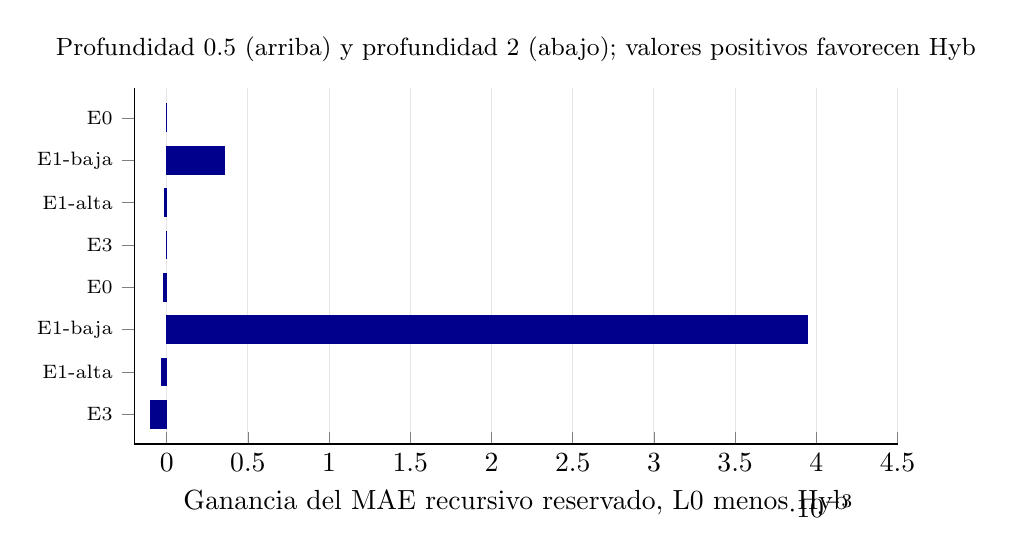
\begin{tikzpicture}
\begin{axis}[
  xbar, width=0.93\textwidth, height=6.1cm,
  xmin=-0.0002, xmax=0.0045,
  xlabel={Ganancia del MAE recursivo reservado, L0 menos Hyb},
  symbolic y coords={C1,C2,C3,C4,C5,C6,C7,C8}, ytick=data,
  yticklabels={E0, E1-baja, E1-alta, E3, E0, E1-baja, E1-alta, E3},
  yticklabel style={font=\scriptsize},
  y dir=reverse, xmajorgrids=true, grid style={gray!20},
  axis x line*=bottom, axis y line*=left,
  title style={font=\small}, title={Profundidad 0.5 (arriba) y profundidad 2 (abajo); valores positivos favorecen Hyb}
]
\addplot[fill=blue!55!black,draw=blue!55!black] coordinates {
  (-0.000002,C1) (0.000354,C2) (-0.000014,C3) (-0.000003,C4)
  (-0.000017,C5) (0.003943,C6) (-0.000033,C7) (-0.000101,C8)
};
\end{axis}
\end{tikzpicture}
\caption{Ganancia media del MAE recursivo del error de precio por condición operativa y profundidad. Cada barra promedia cuatro magnitudes de choque reservadas; los contrastes por celda son descriptivos y no tienen intervalos de confianza separados. Los valores se exportan en \code{figures/data/hybrid\_depth\_condition.csv}.}
\label{fig:hybrid-cell-gains}
\end{figure}

El promedio primario no debe interpretarse aisladamente: casi toda la ganancia proviene de una combinación de baja capacidad y profundidad, mientras que la predicción de la presión de flujo no mejora. El siguiente paso de modelado consiste en representar explícitamente los límites de capacidad y las transiciones de retiro de LP y evaluarlos con otro protocolo congelado, en vez de añadir más términos polinómicos libres. La comparación de mapas es un diagnóstico predictivo de un modelo sustituto. No establece una función de Lyapunov, estabilidad local del mapa por tramos ni estabilidad estocástica del simulador completo.

\section{Trayectorias por profundidad}

La figura~\ref{fig:prof} compara E1-alta y E3 con $\kappa=0.5$. Con la menor profundidad, E3 parte del mismo exceso inicial y se corrige más despacio. Una explicación compatible es que el retiro deja una piscina más pequeña y que la orden de arbitraje, acotada por $c\,x$, es entonces menor; esta explicación no se contrastó por separado. Con $\kappa=1$ y $2$ las dos trayectorias son casi idénticas. El retorno sostenido ocurre en promedio en el tick $7.8$ para E3 con $\kappa=0.5$ frente a $2.8$ para E1-alta, mientras que con $\kappa=1$ y $2$ las diferencias son de $0.1$ ticks o menos.

\begin{figure}[htbp]
\centering
\begin{tikzpicture}
\begin{axis}[width=0.9\textwidth,height=6.2cm,xlabel={Tick},ylabel={$|d_t|$ medio},grid=major,legend style={font=\scriptsize},xmin=0,xmax=20,ymin=0]
\addplot[thick,blue!70!black] table[col sep=comma,x=tick,y=mean_abs_excess,restrict expr to domain={\thisrow{series_id}}{31:31}] {\datadir/trajectories.csv};
\addplot[thick,dashed,green!50!black] table[col sep=comma,x=tick,y=mean_abs_excess,restrict expr to domain={\thisrow{series_id}}{41:41}] {\datadir/trajectories.csv};
\legend{E1-alta,E3}
\end{axis}
\end{tikzpicture}
\caption{Exceso de error medio con $\kappa=0.5$: arbitraje alto estático (E1-alta) y con retiro adaptativo (E3).}
\label{fig:prof}
\end{figure}

\section{Sensibilidad de ingeniería: recuperación y escala de las órdenes}
\label{sec:engineering-sensitivity}

Un análisis suplementario (análisis 0.6.0, ejecución \code{\EngineeringRunID}) usó 300 semillas nuevas (2000--2299), tres variantes de flujo de órdenes y las 15 celdas de profundidad/choque/condición del diseño confirmatorio congelado: 40\,500 trayectorias de 20 ticks abstractos. Es un análisis descriptivo de sensibilidad, no un nuevo contraste confirmatorio. La recuperación significa el primer par observado de ticks consecutivos dentro de la banda; las salidas posteriores se contabilizan por separado. Los plazos se expresan en ticks, no en tiempo transcurrido.

Con los tamaños absolutos originales, E3 adaptativo se recuperó al menos una vez en el 97.4\,\% de las trayectorias, pero solo el 81.9\,\% terminó dentro de la banda. De las trayectorias que se recuperaron, el 31.2\,\% salió después. Con profundidad 0.5, solo el 45.8\,\% terminó dentro de la banda y el 98.8\,\% de las trayectorias recuperadas salió posteriormente. Por tanto, en este modelo, un primer retorno sostenido no equivale a un seguimiento persistente. Estos promedios igualmente ponderados del diseño no sustentan una afirmación poblacional con ajuste por multiplicidad.

El contraste de respuesta máxima entre E3 adaptativo y estático cambia según la definición de las órdenes (tabla~\ref{tab:engineering-sensitivity}). Mantener fijos los tamaños absolutos produjo un efecto con profundidad 0.5; al escalar las órdenes de ruido y tendencia con las reservas iniciales, el contraste fue efectivamente cero en las tres profundidades. Desactivar la venta de pánico redujo el contraste de baja profundidad, pero no lo eliminó. Esto aísla un límite importante del modelo: la profundidad por sí sola no determina el resultado; también importan el tamaño de la orden relativo a las reservas y la regla de reacción.

\begin{table}[htbp]
\centering
\caption{Respuesta máxima suplementaria pareada: E3 adaptativo menos estático por profundidad (300 semillas nuevas). Intervalos aproximados del 95\,\% sin ajuste.}
\label{tab:engineering-sensitivity}
\small
\begin{tabular}{@{}lrrr@{}}
\toprule
Variante del flujo de órdenes & Profundidad 0.5 & Profundidad 1 & Profundidad 2 \\
\midrule
Órdenes absolutas fijas & 0.03458 [0.03225, 0.03690] & 0.00000 & 0.00000 \\
Órdenes proporcionales a reservas iniciales & 0.00000 & 0.00000 & 0.00000 \\
Órdenes fijas, sin pánico & 0.01471 [0.01364, 0.01577] & 0.00000 & 0.00000 \\
\bottomrule
\end{tabular}
\end{table}

Con profundidad 0.5 y órdenes absolutas fijas, E3 adaptativo terminó dentro de la banda en el 45.8\,\% de las trayectorias; con órdenes proporcionales, terminó dentro en el 100\,\%. Estas variantes comparten el mismo modelo estilizado de agentes representativos y no constituyen comparaciones empíricas. Los resúmenes por celda, contrastes pareados, configuración y hashes completos se exportan en \code{figures/engineering/}.

\section{Piloto exploratorio de ingesta de datos DEX (no confirmatorio)}
\label{sec:dex-pilot-results}

El extracto público de DEX contiene tres intercambios WETH/USDT dentro de una ventana de captura de seis minutos. El volumen cotizado sumado es 1,856.56 USDT, y los precios efectivos de intercambio van de 1,703.11 a 1,703.97 USDT/ETH (tabla~\ref{tab:dex-pilot}). Las estimaciones de deslizamiento de la fuente para tamaños hipotéticos van de 0.0216\,\% a 0.0362\,\% para una operación de 1,000 USDT, y de 0.1697\,\% a 0.1843\,\% para una de 10,000 USDT. El nivel nominal de comisión del pool es 0.30\,\%. Estos valores describen tres eventos del extracto; no estiman la actividad total del mercado ni un resultado de series temporales.

Los campos de deslizamiento son estimaciones de la fuente para tamaños hipotéticos; no son costos realizados por el agente de la tesis. La comisión nominal del pool excluye el gas y los costos específicos de una cuenta en un CEX. Aunque una ejecución local de ingesta generó una alineación por minuto con un flujo CEX, aquí no se informan observaciones derivadas del CEX ni diferencias de precios porque sus derechos de redistribución no están resueltos. Por tanto, este piloto comprueba únicamente la adquisición de datos y el tratamiento de campos. La muestra es demasiado breve y fue seleccionada para inspeccionar la tubería; no permite probar el seguimiento, el arbitraje, la recuperación, la latencia ni las comisiones en operación real, y no cambia H1--H3.

\begin{table}[htbp]
\centering
\caption{Resumen descriptivo de la muestra DEX abierta del piloto (tres intercambios; no confirmatorio).}
\label{tab:dex-pilot}
\small
\begin{tabularx}{\textwidth}{@{}>{\raggedright\arraybackslash}p{0.30\textwidth}>{\raggedright\arraybackslash}p{0.25\textwidth}X@{}}
\toprule
Medida & Valor de la muestra & Interpretación \\
\midrule
Intercambios observados & 3 & Eventos del extracto en una ventana de captura de seis minutos \\
Volumen cotizado sumado & 1,856.56 USDT & Suma de los tres eventos únicamente \\
Precio efectivo de intercambio & 1,703.11--1,703.97 USDT/ETH & Precios de los eventos, no precios marginales implícitos en las reservas \\
Estimación de deslizamiento & 0.0216--0.0362\,\% a 1,000 USDT & Estimación para tamaño de operación hipotético \\
Estimación de deslizamiento & 0.1697--0.1843\,\% a 10,000 USDT & Estimación para tamaño de operación hipotético \\
Nivel nominal de comisión del pool & 0.30\,\% & Excluye gas y costos del CEX \\
\bottomrule
\end{tabularx}
\end{table}

La tabla se regenera desde el extracto público incluido con \code{analyze\_dex\_pilot.py}; la muestra y su procedencia se documentan en \code{data/samples/empirical-pilot/README.md}.

\section{Resumen de los resultados}

\begin{itemize}
  \item \textbf{H1:} se rechaza la nula; el arbitraje activo reduce el área de exceso en $2.26$ en promedio y la capacidad gradúa la recuperación. La precisión objetivo no se alcanzó con 300 semillas.
  \item \textbf{H2:} se rechaza la nula en promedio, con $\Delta_2=0.0114$, pero el efecto existe solo con $\kappa=0.5$ y la mitad aproximada del efecto depende del agente de pánico.
  \item \textbf{H3:} se rechaza la nula frente a la persistencia, pero el mapa no supera a un autorregresivo escalar, no mejora a la persistencia en E0 y su clasificación de regímenes es débil.
  \item \textbf{Sensibilidad de ingeniería:} el retorno puede ser temporal (el 31.2\,\% de las trayectorias E3 recuperadas sale luego de la banda en el agregado); el contraste H2 de poca profundidad desaparece al escalar las órdenes con las reservas y se reduce al desactivar el pánico.
  \item \textbf{Disponibilidad de datos reales:} el piloto de tres intercambios DEX demuestra que se puede ingerir y resumir un extracto abierto pequeño; no aporta validación de mercado ni evidencia para H1--H3.
\end{itemize}
